%%\documentclass[a4paper, 12pt]{scrreprt}

\documentclass[a4paper, 12pt]{scrartcl}
%usepackage[german]{babel}
\usepackage{microtype}
%\usepackage{amsmath}
%usepackage{color}
\usepackage[utf8]{inputenc}
\usepackage[T1]{fontenc}
\usepackage{wrapfig}
\usepackage{lipsum}% Dummy-Text
\usepackage{multicol}
\usepackage{alltt}
%%%%%%%%%%%%bis hierhin alle nötigen userpackage
\usepackage{tabularx}
\usepackage[utf8]{inputenc}
\usepackage{amsmath}
\usepackage{amsfonts}
\usepackage{amssymb}

%\usepackage{wrapfig}
\usepackage[ngerman]{babel}
\usepackage[left=25mm,top=25mm,right=25mm,bottom=25mm]{geometry}
%\usepackage{floatrow}
\setlength{\parindent}{0em}
\usepackage[font=footnotesize,labelfont=bf]{caption}
\numberwithin{figure}{section}
\numberwithin{table}{section}
\usepackage{subcaption}
\usepackage{float}
\usepackage{url}
%\usepackage{fancyhdr}
\usepackage{array}
\usepackage{geometry}
%\usepackage[nottoc,numbib]{tocbibind}
\usepackage[pdfpagelabels=true]{hyperref}
\usepackage[font=footnotesize,labelfont=bf]{caption}
\usepackage[T1]{fontenc}
\usepackage {palatino}
%\usepackage[numbers,super]{natbib}
%\usepackage{textcomp}
\usepackage[version=4]{mhchem}
\usepackage{subcaption}
\captionsetup{format=plain}
\usepackage[nomessages]{fp}
\usepackage{siunitx}
\sisetup{exponent-product = \cdot, output-product = \cdot}
\usepackage{hyperref}
\usepackage{longtable}
\newcolumntype{L}[1]{>{\raggedright\arraybackslash}p{#1}} % linksbündig mit Breitenangabe
\newcolumntype{C}[1]{>{\centering\arraybackslash}p{#1}} % zentriert mit Breitenangabe
\newcolumntype{R}[1]{>{\raggedleft\arraybackslash}p{#1}} % rechtsbündig mit Breitenangabe
\usepackage{booktabs}
\renewcommand*{\doublerulesep}{1ex}
\usepackage{graphicx}


\usepackage[backend=bibtex, style=chem-angew, backref=none, backrefstyle=all+]{biblatex}
\bibliography{Literatur.bib}
\defbibheading{head}{\section{Literatur}\label{sec:Lit}} 
\let\cite=\supercite
%\begin{document}
%\setlength\abovedisplayshortskip{20pt}
%\setlength\belowdisplayshortskip{20pt}
%\setlength\abovedisplayskip{20pt}
%\setlength\belowdisplayskip{20pt}
\section {Auswertung}

Es wurde ein Rotationsschwingungsspektrum \ref{Spektrum} von CO mittels eines Fourier-Transform-Infrarot-Spektrometer (FTIR-Spektrometer) aufgenommen.

\begin{figure}[H]
	\centering	
	\begin{minipage}{1\textwidth}
		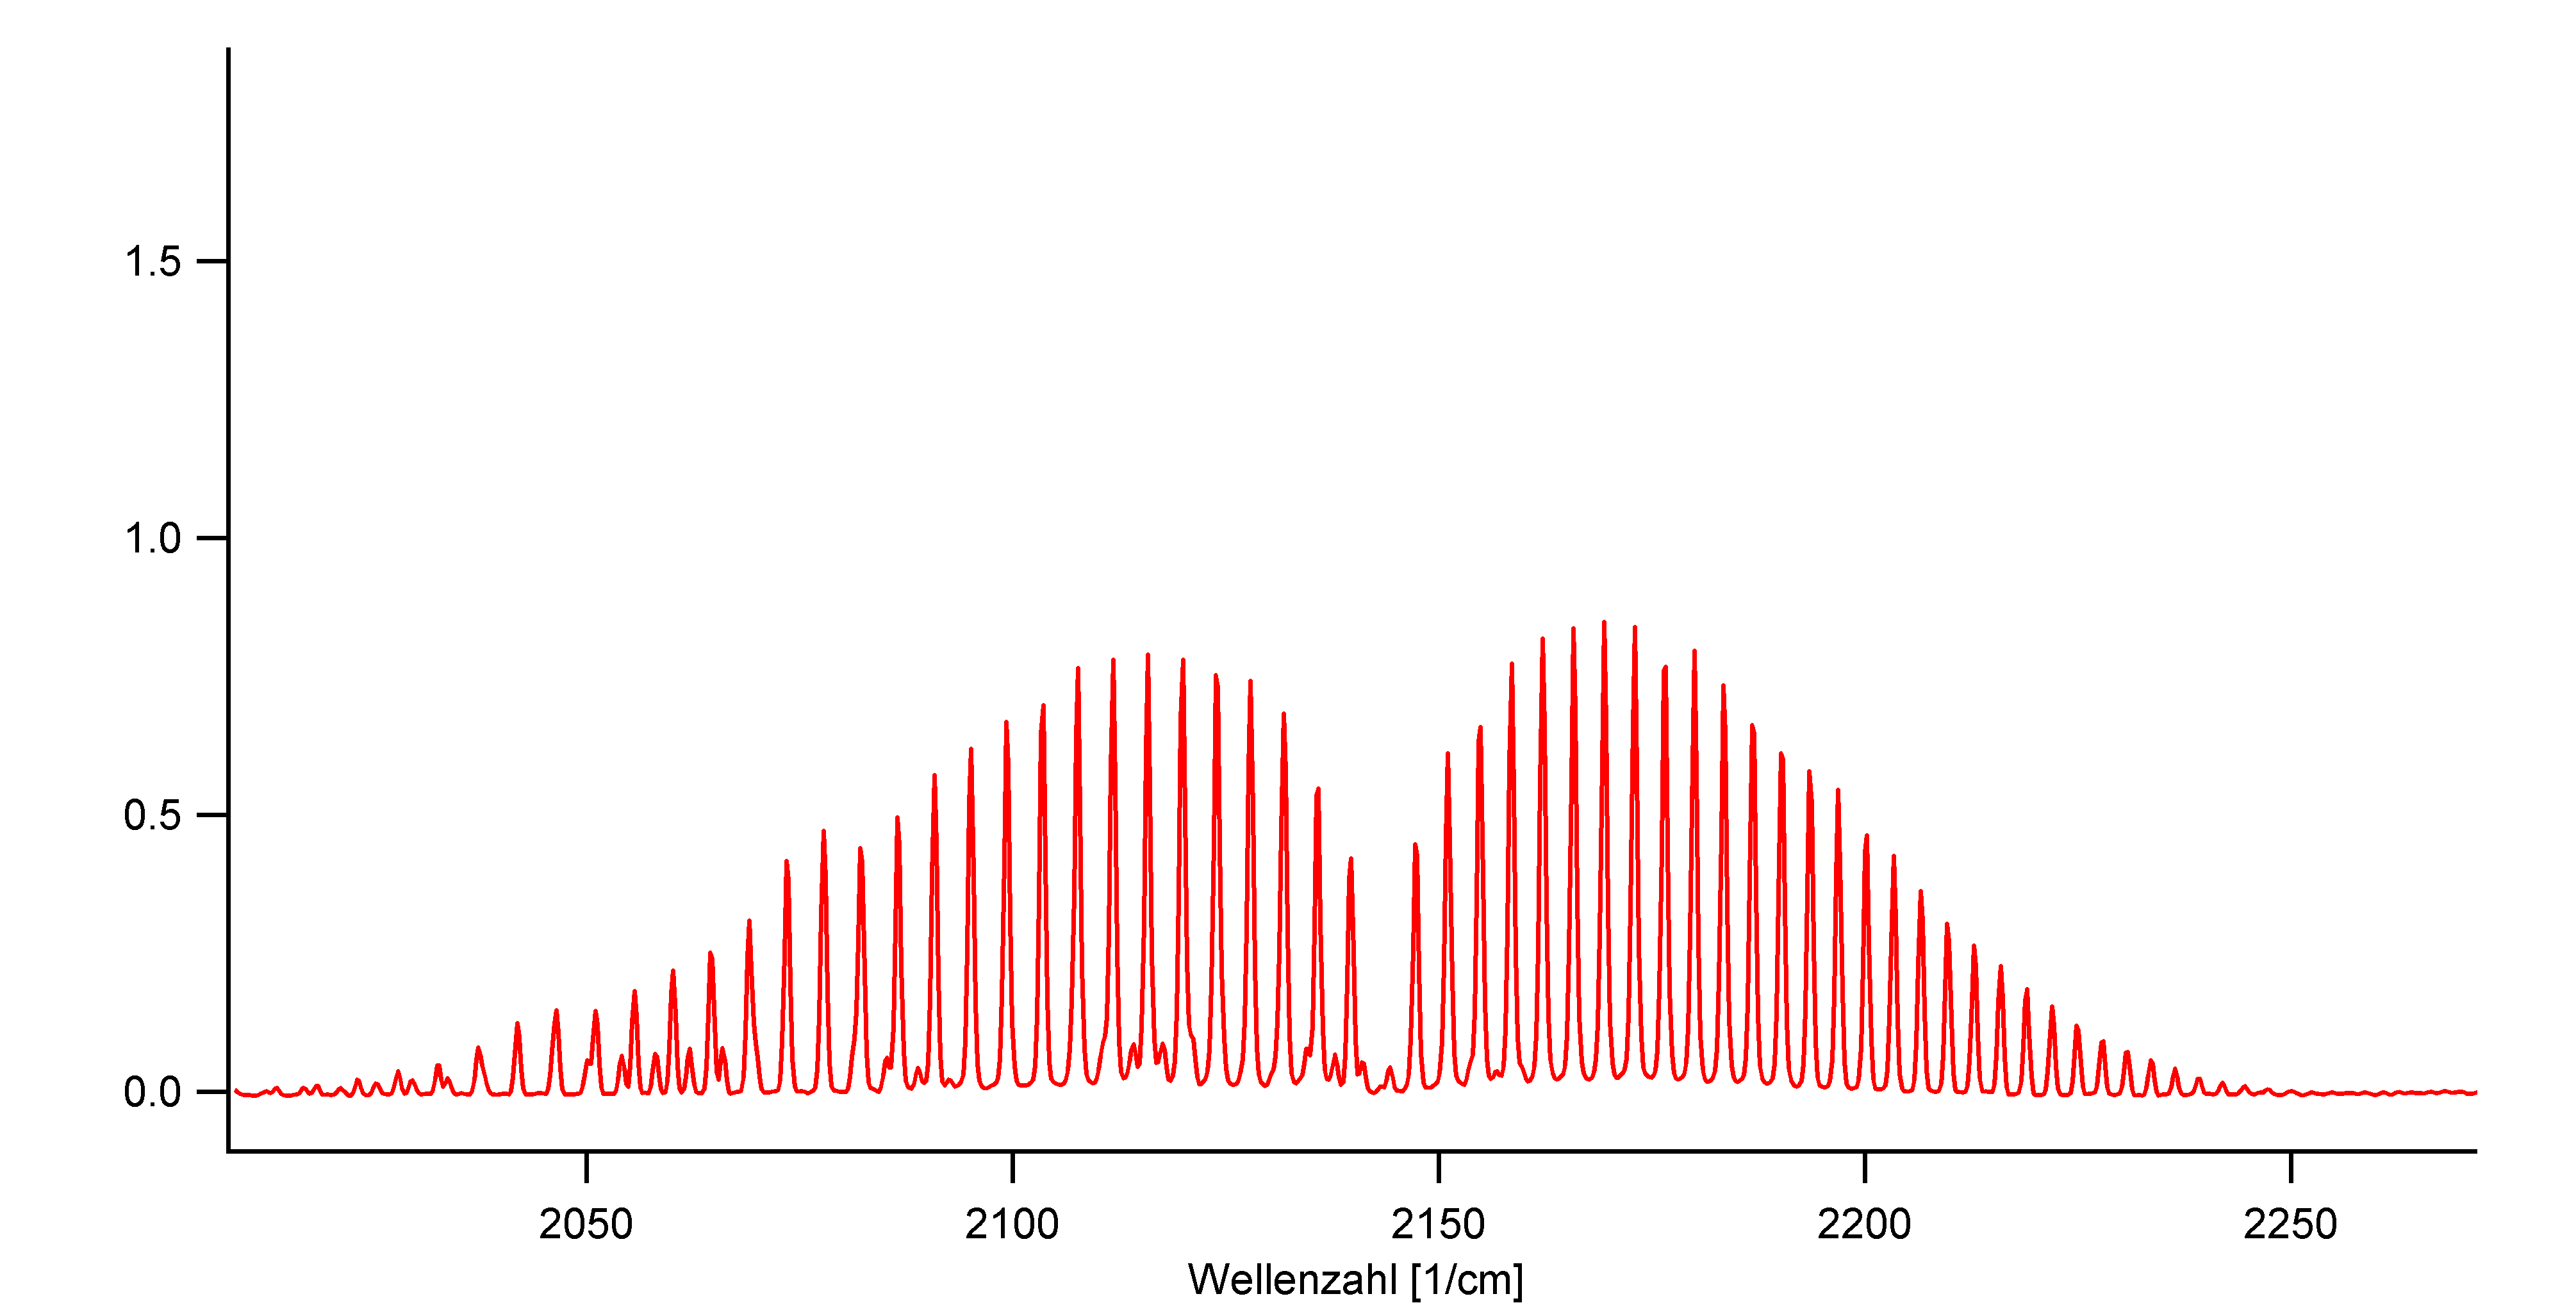
\includegraphics[width=\columnwidth]{Bilder/Graph_spektrum.png}
	\end{minipage}
	\caption{Rotationsschwingungspektrum von CO. Die Daten wurden mit einem FTIR-Spektrometer aufgenommen und mit Igor Pro dargestellt }
	\label{Spektrum}
\end{figure}
Mit dem Igor Pro Peak-Picker wurden die lokalen Maxima des Spektrums gefunden, welche in Tabelle \ref{Tabelle} dargestellt sind. Bei rund 2143~$cm^{-1}$ befindet sich die Nulllücke. Die Peaks bei höheren bzw niedrigeren Wellenzahlen werden entsprechend positiv bzw. negativ mit der Laufzahl $m$ durchnummeriert.

\begin{table}[H]
\centering

	\caption{Wellenzahl, Intensiät und Laufzahl des Rotationsspektrums von CO. Die Auswertung der Daten erfolgten mit Igor Pro. }
	\begin{tabular}{C{0.15\linewidth}|C{0.15\linewidth}|C{0.15\linewidth}}
		Wellenzahl [$cm^{-1}$] & Intesität & Laufzahl $m$\\
		\hline \addlinespace[1ex] 
$2027.88$&	$0.0298$&	$-27$\\
$2032.7$&	$0.0419245$&	$-26$\\
$2037.28$&	$0.0800963$&	$-25$\\
$2041.86$&	$0.108158$&	$-24$\\
$2046.2$&	$0.13768$&	$-23$\\
$2050.78$&	$0.12754$&	$-22$\\
$2055.36$&	$0.143957$&	$-21$\\
$2059.94$&	$0.175645$&	$-20$\\
$2064.52$&	$0.218814$&	$-19$\\
$2069.1$&	$0.269178$&	$-18$\\
$2073.44$&	$0.362985$&	$-17$\\
$2077.78$&	$0.409497$&	$-16$\\
$2082.12$&	$0.405746$&	$-15$\\
\label{Tabelle}
	\end{tabular}
\end{table}
\begin{table}[H]
\centering

	\begin{tabular}{C{0.15\linewidth}|C{0.15\linewidth}|C{0.15\linewidth}}
$2086.46$&	$0.425813$&	$-14$\\
$2090.8$&	$0.4711$&	$-13$\\
$2094.9$&	$0.520347$&	$-12$\\
$2099.24$&	$0.575038$&	$-11$\\
$2103.34$&	$0.603483$&	$-10$\\
$2107.44$&	$0.654823$&	$-9$\\
$2111.54$&	$0.636419$&	$-8$\\
$2115.64$&	$0.61416$&	$-7$\\
$2119.73$&	$0.668546$&	$-6$\\
$2123.83$&	$0.682587$&	$-5$\\
$2127.69$&	$0.622256$&	$-4$\\
$2131.55$&	$0.600051$&	$-3$\\
$2135.65$&	$0.459026$&	$-2$\\
$2139.5$&	$0.346856$&	$-1$\\
$2143.84$&	$0.0266294$&	$0$\\
$2147.22$&	$0.390804$&	$1$\\
$2150.84$&	$0.520884$&	$2$\\
$2154.69$&	$0.569379$&	$3$\\
$2158.31$&	$0.638937$&	$4$\\
$2162.17$&	$0.68343$&	$5$\\
$2165.78$&	$0.699162$&	$6$\\
$2169.4$&	$0.711813$&	$7$\\
$2172.78$&	$0.690448$&	$8$\\
$2176.39$&	$0.672499$&	$9$\\
$2179.77$&	$0.664652$&	$10$\\
$2183.38$&	$0.617512$&	$11$\\
$2186.76$&	$0.579296$&	$12$\\
$2190.13$&	$0.53833$&	$13$\\
$2193.51$&	$0.494124$&	$14$\\
$2196.89$&	$0.458531$&	$15$\\
$2200.02$&	$0.398535$&	$16$\\
$2203.39$&	$0.361041$&	$17$\\
$2206.53$&	$0.305348$&	$18$\\
$2209.66$&	$0.259686$&	$19$\\
$2212.8$&	$0.22201$&	$20$\\
$2215.93$&	$0.194417$&	$21$\\
$2218.82$&	$0.162487$&	$22$\\
$2221.96$&	$0.132927$&	$23$\\
$2224.85$&	$0.107074$&	$24$\\
$2227.75$&	$0.0835625$&	$25$\\
$2230.64$&	$0.0688465$&	$26$\\
$2233.53$&	$0.05248$&	$27$\\
$2236.43$&	$0.0380294$&	$28$\\
$2239.08$&	$0.0252758$&	$29$\\

	
	\end{tabular}
\end{table}

Durch Auftragen der Wellenzahlen gegen die Laufzahl der Peaks und eine Polynomregression zweiten Grades erhält man die exakte Position der Nulllücke sowie die Summe als auch die Differenz der Roationskonstanten vom Grundzustand und  vom angeregten Zustand.


\begin{figure}[H]
	\centering	
	\begin{minipage}{1\textwidth}
		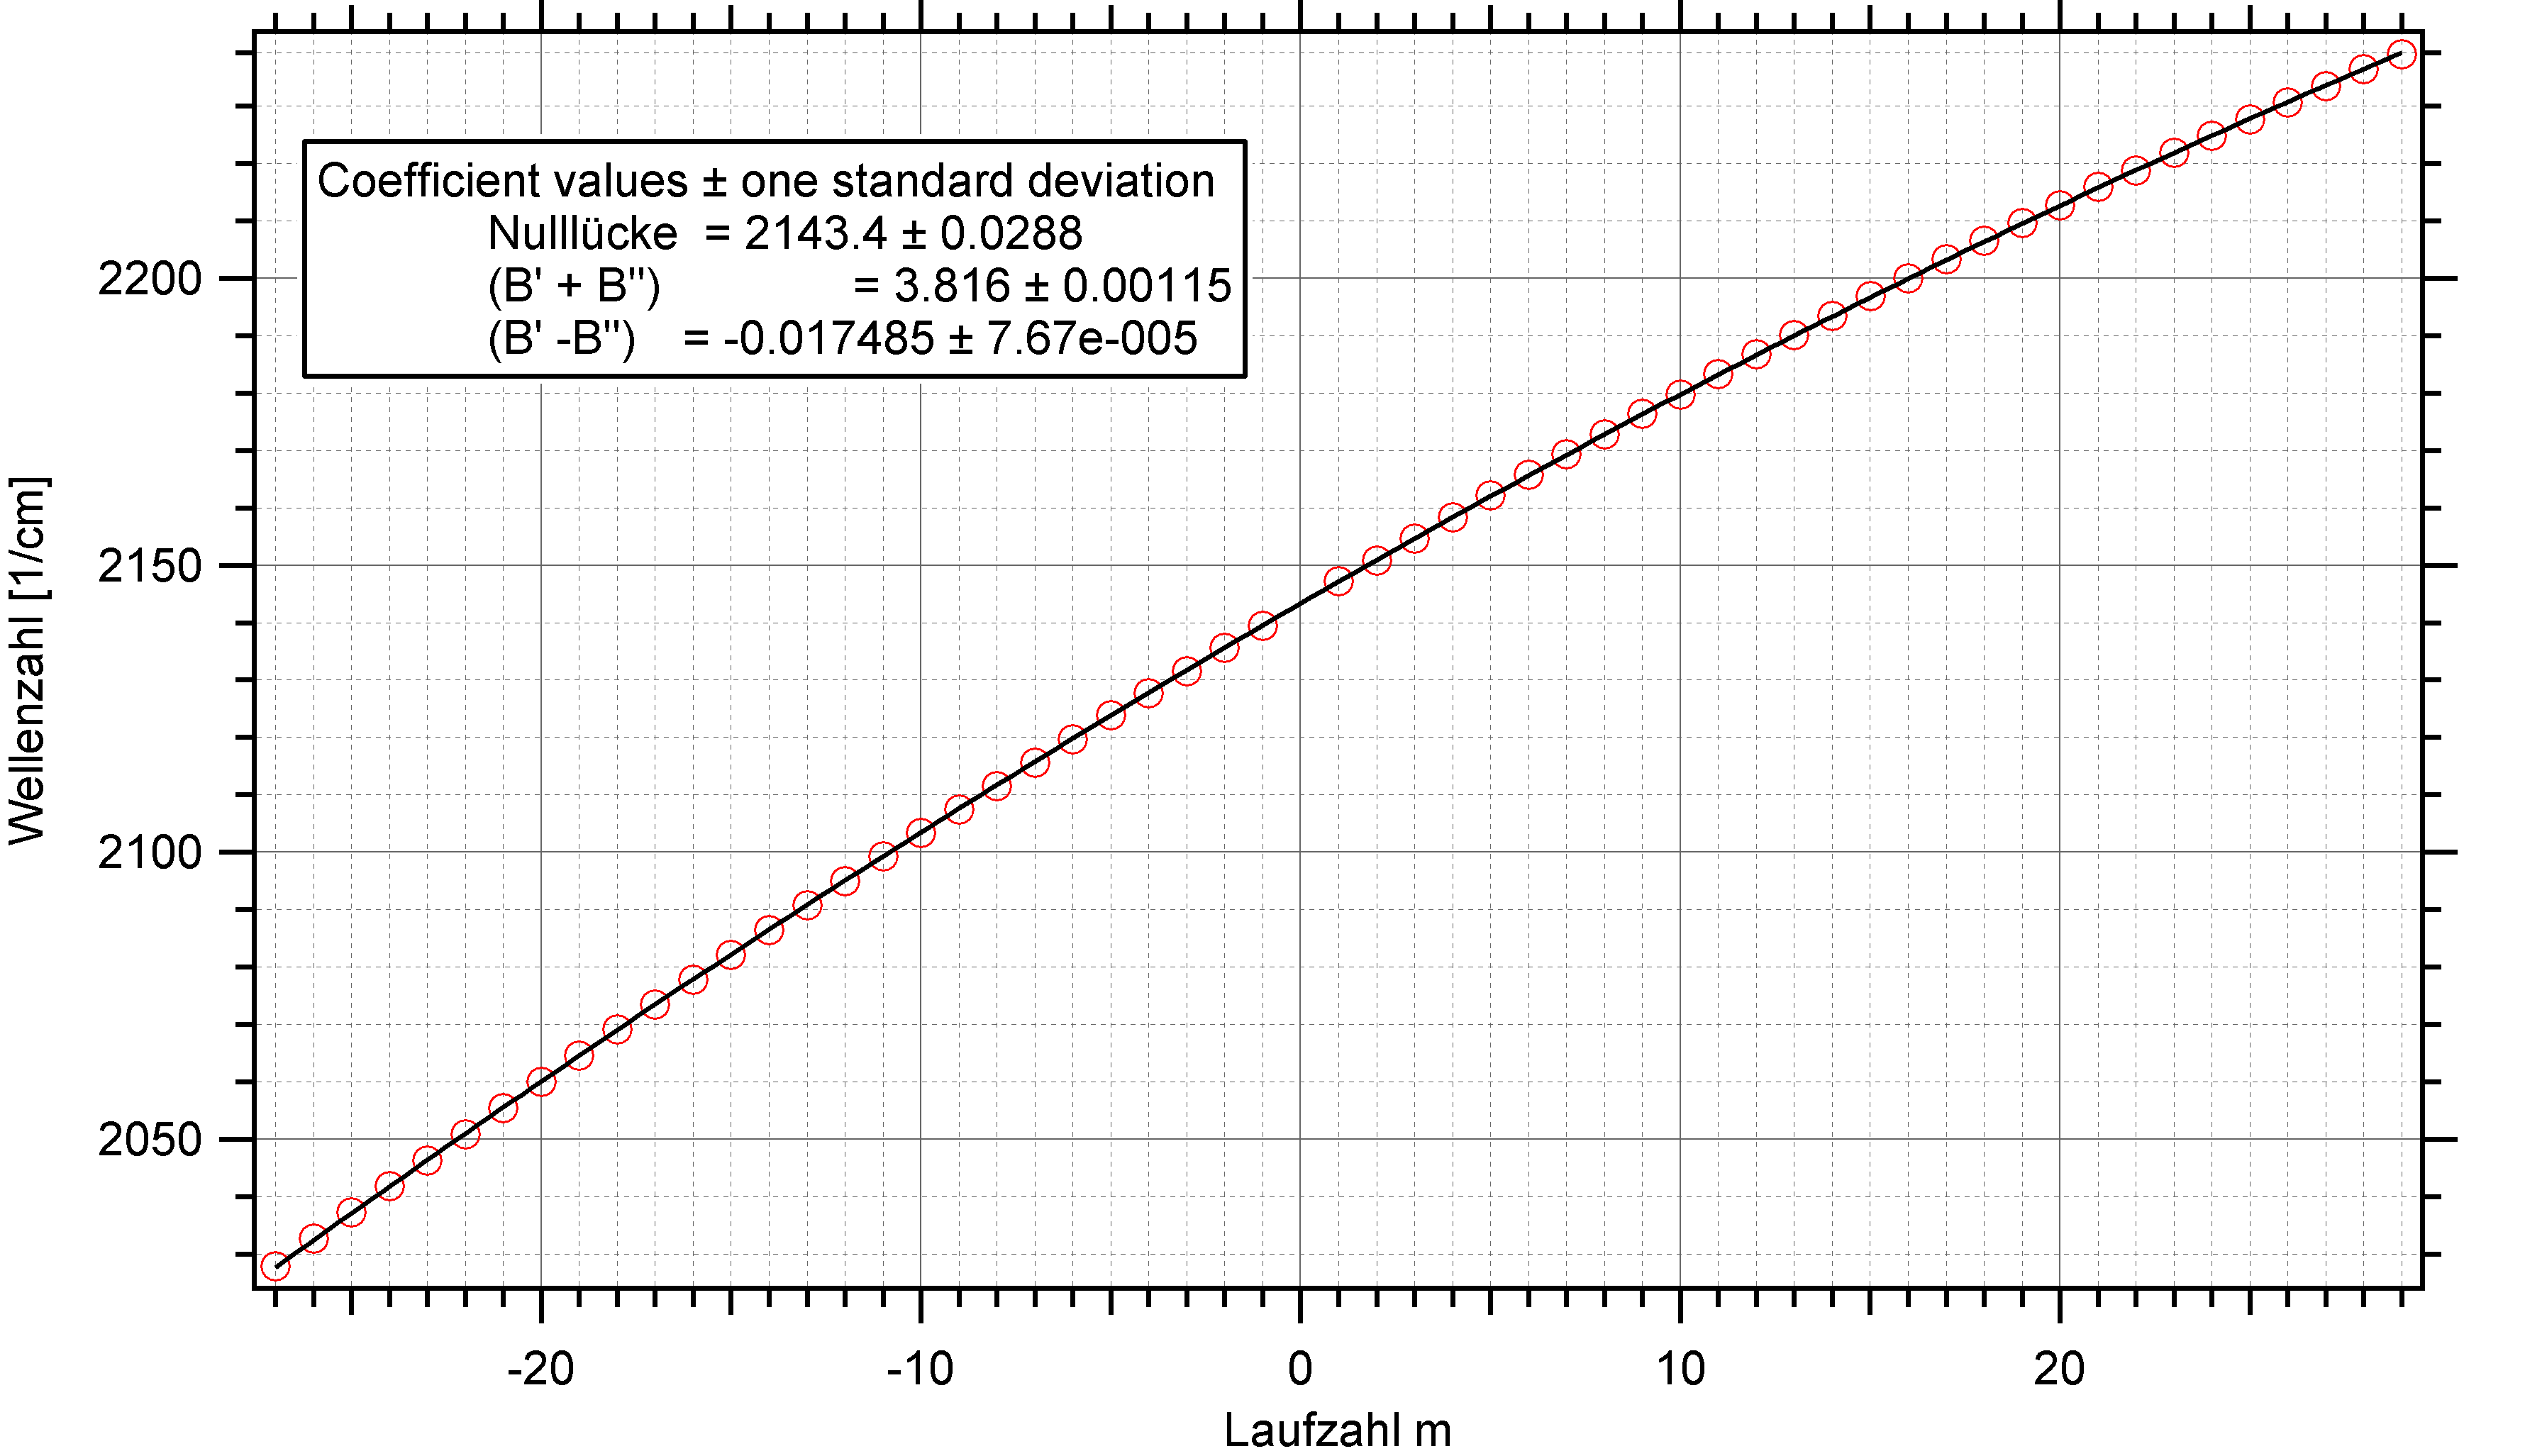
\includegraphics[width=\columnwidth]{Bilder/Graph_fitm.png}
	\end{minipage}
	\caption{Auftragung der Wellenzahlen der Peaks des Rotationsschwingungspektrum von CO über der Laufzahl. Die Daten wurden mit mit Igor Pro dargestellt und mit einem Polynom zweiten Grades angepasst.}
	\label{fit3}
\end{figure}

Aus den in der  Regression erhaltenen Werten lassen sich nun $B_0$ und $B_1$ und daraus gemäß Formel \ref{for:be} $B_e$ berechen.


\begin{equation}
B_e=B_0+\frac{\alpha_e}{2}\quad\quad \textit{mit}\quad \alpha_e=B_0-B_1
\label{for:be}
\end{equation}

Allgemein gilt: 
\begin{equation}
B=\frac{h}{8\pi^2\cdot c\cdot \mu \cdot r^2}\quad\quad \textit{mit}\quad \mu=\frac{m_Cm_O}{m_C+m_O}
\end{equation}

Dies kann man nun nach $r$ umstellen und die entsprechenden Werte für $B$ einsetzten um die Abstände zu erhalten.

\begin{equation}
r=\sqrt{\frac{h}{8\pi^2\cdot c\cdot \mu \cdot B}}
\end{equation}

Alle entsprechend den obigen Gleichungen berechneten Werte sind in Tabelle \ref{Zusammenfassung} zusammengefasst. Alle Werte liegen außerhalb des doppelten Fehlerintervalls und sind somit als nicht richtig zu bewerten, jedoch stimmt die Größenordnung. Mögliche Gründe für die Abweichungen können durchGerätefehler bzw. systematische Fehler in der Regression zustande gekommen sein. Gerade die Anpassung durch das quadratische Polnom durch Igor ist nur eine Näherung, dessen Qualität sich jedoch nur schwer bewerten lässt.

\begin{table}
\label{Zusammenfassung}
	\caption{Zusammenfassung der berechneten Konstanten aus dem Rotationsschwingungspektrum von CO.  }
\begin{tabular}{C{0.2\linewidth}|C{0.2\linewidth}|C{0.2\linewidth}|C{0.2\linewidth}}
Konstante             & Einheit                  & Wert                           & Literatur\cite{Lit} \\ \hline
$B_0$                  & [$cm^{-1}$]          & $1.9167 \pm 0.0006$	& $1.68172$   \\
$B_1$                  & [$cm^{-1}$]          & $1.896 \pm 0.002$   	& $1.66268$   \\
$B_e $                 & [$cm^{-1}$]          & $1.927 \pm 0.002$   	& $1.69124$   \\
$\alpha$		& [$cm^{-1}$]       & $0.081 \pm 0.003$   	& $0.01904$   \\
$r_e$                  & $\SI{}{[\angstrom]}$		& $1.129 \pm 0.0012 $  	& $1.206$     \\
$r_0$                  & $\SI{}{[\angstrom]} $		& $1.132 \pm 0.004$  	 & $1.209$     \\
$r_1$                  & $\SI{}{[\angstrom]}$ 		& $1.138 \pm 0.004$  	 & $1.216$    \\
$\nu_0$	&[$cm^{-1}$]          & $2143.40 \pm 0.03$&
\end{tabular}
\end{table}


Da die Rotationskonstanten additiv bzw subtraktiv miteinander verknüpft sind, entsprechen die Fehler der Addition der aboluten Fehler, welche aus den Anpassungen in Igor entnommen wurden. 



%\end{document}

